% Author: Izaak Neutelings (July 2017)
% Sources:
%  https://www.tandfonline.com/doi/abs/10.1080/14786440508637080
%  https://indico.cern.ch/event/1126814/contributions/4729554/attachments/2386887/4079372/Izaak_paper_reading_Rutherford_nucleus_20170713_v5.pdf
\documentclass[border=3pt,tikz]{standalone}
\usepackage{amsmath} % for \dfrac
\usepackage{tikz}
\tikzset{>=latex} % for LaTeX arrow head
\usepackage{pgfplots} % for the axis environment
\usetikzlibrary{calc} % to do arithmetic with coordinates
\usetikzlibrary{angles,quotes} % for pic
\usetikzlibrary{arrows.meta} % for arrow size
\usetikzlibrary{bending} % for arrow head angle
\tikzstyle{bend>}=[-{Latex[flex'=1,length=3,width=2.5]}]
\tikzstyle{<bend}=[{Latex[flex'=1,length=3,width=2.5]}-]

% colors
%\definecolor{mylightblue}{RGB}{170,170,230}
\definecolor{mylightgrey}{RGB}{230,230,230}
\definecolor{mygrey}{RGB}{190,190,190}
\definecolor{mydarkgrey}{RGB}{110,110,110}
\definecolor{mygreen}{RGB}{120,220,160}
\definecolor{mydarkgreen}{RGB}{60,120,60}
\definecolor{myverydarkgreen}{RGB}{35,90,35}
\definecolor{mydarkred}{RGB}{140,40,40}
\definecolor{mylightblue}{RGB}{220,228,255}
\definecolor{myblue}{RGB}{183,191,229}
\definecolor{mydarkblue}{RGB}{50,70,190}
\definecolor{mygold}{RGB}{250,200,80}

% mark right angle
\newcommand{\MarkRightAngle}[4][1.3mm]{
  \coordinate (tempa) at ($(#3)!#1!(#2)$);
  \coordinate (tempb) at ($(#3)!#1!(#4)$);
  \coordinate (tempc) at ($(tempa)!0.5!(tempb)$);%midpoint
  \draw (tempa) -- ($(#3)!2!(tempc)$) -- (tempb);
}

\begin{document}


% RUTHERFORD SCATTERING
\begin{tikzpicture}[scale=1]
  \message{^^JRutherford scattering}
  
  % limits & parameters
  \def\xa{-2.4}
  \def\xb{ 4}
  \def\ya{-4}
  \def\yb{ 4}
  \def\tmax{2.1}
  \def\a{1.3}
  \def\b{1}
  \def\c{{sqrt(\a^2+\b^2)}}
  \def\N{50} % number of points
  
  % coordinates
  \coordinate (O)  at ( 0,0);
  \coordinate (A)  at (\a,0);
  \coordinate (F1) at ( {sqrt(\a^2+\b^2)},0);
  \coordinate (F2) at (-{sqrt(\a^2+\b^2)},0);
  \coordinate (P)  at (-{\a^2/sqrt(\a^2+\b^2)},-{\a*\b/sqrt(\a^2+\b^2)});
  \coordinate (P1) at (\xb*\a, \yb*\b);
  \coordinate (P2) at (\xb*\a,-\yb*\b);
  \coordinate (yshift) at (0,0.4);
  
  % axes & asymptotes
  \draw[mygrey] % x axis
    (\xa*\a,0) -- (\xb*\a,0);
  %\draw[mylightgrey] % y axis
  %  (0,\ya*\b) -- (0,\yb*\b);
  \draw[dashed,mydarkgrey]
    (-\xb*\a*0.45, \ya*\b*0.45) -- (\xb*\a, \yb*\b)
    (-\xb*\a*0.45,-\ya*\b*0.45) -- (\xb*\a,-\yb*\b);
  
  % arrows
  \def\vtheta{30}
  \def\vradius{0.8}
  \draw[->,myverydarkgreen,shift=($(P1)-(yshift)$),scale=0.6]
	(0,0) -- (-\a,-\b) node[midway,below right=0pt] {${v}_i$};
  \draw[->,myverydarkgreen,shift=($(P2)+(yshift)$),scale=0.6]
	(-\a,\b) -- (0,0) node[midway,above right=-2pt] {${v}_f$};
  \draw[->,myverydarkgreen]
    (\a+0.35,{\vradius*sin(\vtheta)}) arc (180-\vtheta:180+\vtheta+10:\vradius)
    node[above right=0pt] {$v^*$};
  
  % angles
  \MarkRightAngle[2.0mm]{F2}{P}{O}
  \pic[draw,myverydarkgreen,"$\theta$",angle radius=13,angle eccentricity=1.35] {angle=F2--O--P};
  \pic[draw,bend>,myverydarkgreen,"$\phi$"{scale=1,anchor=100,inner sep=4.5},angle radius=10] {angle=P--O--P2};
  
  % hyperbola
  \draw[color=mylightgrey,line width=0.5,samples=\N,smooth,variable=\t,domain=-\tmax*0.58:\tmax*0.58] % left
    plot({-\a*cosh(\t)},{\b*sinh(\t)});
  \draw[color=mydarkgreen,line width=1,samples=\N,smooth,variable=\t,domain=-\tmax:\tmax] % right
    plot({ \a*cosh(\t)},{\b*sinh(\t)}); % {exp(\y)+exp(-\y)
  
  % nodes
  \draw[myverydarkgreen]
    (F2) -- (P)
    node[midway,below left=1,circle,fill=white,inner sep=-0.2] {$b$};
  \fill
  	%(F1) circle node[above] {F}
    (A) circle(1.5pt) node[above left=0] {A}
    (O) circle(1.5pt) node[above=2pt] {O};
  \fill[mydarkred]
    (F2) circle(4.0pt) node[anchor=-60,inner sep=5] {N};
  \node[left=1pt,above=-1] at ($(F2)!0.5!(O)$) {$c$};
  \node[below right=-2] at ($(P)!0.4!(O)$) {$a$};
  
  % alpha particle
  \draw[mydarkgreen,fill]
    ({ \a*cosh(\tmax*1.02)},{\b*sinh(\tmax*1.02)}) circle(1pt)
    node[above right=0pt] {$\alpha$};
  
\end{tikzpicture}


% RUTHERFORD SCATTERING - backscattering
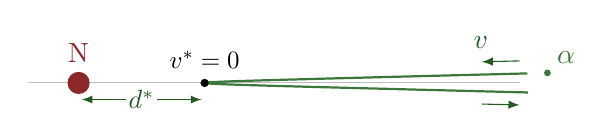
\begin{tikzpicture}[scale=1]
  \message{^^JBack scattering}
  
  % limits & parameters
  \def\xa{-1.8}
  \def\xb{ 6}
  \def\ya{-4}
  \def\yb{ 4}
  \def\a{0.8}
  \def\b{0.02}
  \def\tmax{2.5}
  \def\c{{sqrt(\a^2+\b^2)}}
  \def\N{100} % number of points
  
  % coordinates
  \coordinate (O)  at (   0,  0 );
  \coordinate (A)  at (  \a,  0 );
  \coordinate (F2) at ( -{sqrt(\a^2+\b^2)},   0 );
  \coordinate (P1) at (\xb*\a, \yb*\b);
  \coordinate (P2) at (\xb*\a,-\yb*\b);
  \coordinate (yshift) at (0,0.2);
  
  % axes & asymptotes
  \draw[mygrey] % x
    (\xa*\a,0) -- (\xb*\a,0);
    
  % arrows
  \def\vtheta{30}
  \def\vradius{0.8}
  \draw[->,myverydarkgreen,shift=($(P1)+(yshift)$),scale=0.6]
	(0,0) -- (-\a,-\b) node[midway,above left=1pt] {$v$};
  \draw[->,myverydarkgreen,shift=($(P2)-(yshift)$),scale=0.6]
	(-\a,\b) -- (0,0); %node[midway,below right=0pt] {}; %${v}_f$
  
  % hyperbola
  \draw[color=mydarkgreen,line width=0.8,samples=\N,variable=\t,domain=-\tmax:\tmax]
    plot({ \a*cosh(\t)},{\b*sinh(\t)});
  
  % nodes
  \fill
    (A) circle(1.5pt) node[above=2pt,scale=0.9] {$v^*=0$};
  \fill[mydarkred]
    (F2) circle(4.0pt) node[above=4pt] {N};
  \draw[<->,myverydarkgreen,transform canvas={yshift=-6pt,scale=0.95}]
  	(F2) -- (A)
    node[midway,fill=white,inner sep=1] {$d^*$};
  
  % alpha particle
  \draw[mydarkgreen,fill]
    ({ \a*cosh(\tmax*1.02)},{\b*sinh(\tmax*1.02)}) circle(1pt)
    node[above right=0pt] {$\alpha$};
  
\end{tikzpicture}


% RUTHERFORD GOLD FOIL EXPERIMENT - setup
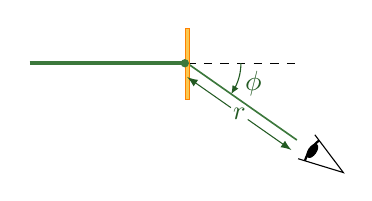
\begin{tikzpicture}[scale=1]
  \message{^^JGold foil experiment}
  
  % limits & parameters
  \def\xa{-2.0} % incoming beam length
  \def\xb{ 1.4} % horizontal line right
  \def\le{0.6}  % eye size eye
  \def\ange{18} % eye opening angle
  \def\lb{1.7}  % outgoing beam length
  \def\ang{-35} % outgoing beam scattering
  \def\h{0.45}  % gold foil height
  \def\w{0.03}  % gold foil width
  
  % coordinates
  \coordinate (A) at (\xa,0);    % incoming beam
  \coordinate (R) at (\xb,0);    % right line
  \coordinate (O) at (  0,0);    % beam hitting foil
  \coordinate (B) at (\ang:\lb); % outgoing beam
  
  % beams
  \draw[dashed] (O) -- (R);
  \draw[mydarkgreen,line width=1.5]
    (A) -- (O);
  \draw[mydarkgreen,line width=0.6]
    (O) -- (B);
  \fill[mygold,draw=orange,line width=0.1] (-\w,-\h) rectangle (\w,\h); % gold foil
  \fill[mydarkgreen]
    (-\w,0) circle(1.5pt);
  
  % angles & distance
  \draw[<->,myverydarkgreen,transform canvas={yshift=-5pt,scale=0.95}]
  	(O) -- (B) node[midway,circle,inner sep=0.5,fill=white] {$r$};
  \pic[draw,<bend,myverydarkgreen,"$\phi$",angle radius=19.4,angle eccentricity=1.29] {angle=B--O--R};
  
  % eye
  \begin{scope}[shift={(\ang:\lb+1.2*\le)},rotate=\ang+180]
    \draw[] (\ange:\le) -- (0,0) -- (-\ange:\le);
    \draw[thick] (\ange:0.85*\le) arc(\ange:-\ange:0.85*\le);
    %\draw[fill,brown] (0.75*\le,0) ellipse ({0.10*\le} and {0.21*\le});
    \draw[fill] (0.8*\le,0) ellipse ({0.08*\le} and {0.16*\le});
  \end{scope}
  
\end{tikzpicture}


% RUTHERFORD SCATTERING - hyperbola triangle
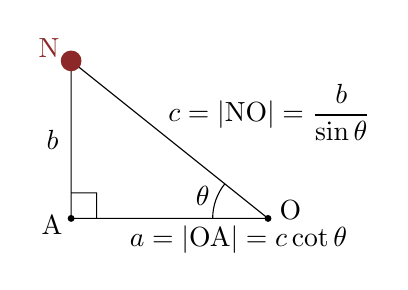
\begin{tikzpicture}[scale=2.5]
  \message{^^JHyperbolic triangle}
  
  % coordinates
  \coordinate (O) at ( 0,0);
  \coordinate (A) at (-1,0);
  \coordinate (B) at (-1,0.8);
  
  % lines
  \draw[]
    (O) -- (A) node[pos=0.15,below=-1] {$a=|\text{OA}|=c\cot\theta$} %\dfrac{c}{\tan(\theta)}
        -- (B) node[pos=0.5,left=1]  {$b$}
        -- (O) node[pos=0.5,above right=-4] {$c=|\text{NO}|=\dfrac{b}{\sin\theta}$};
  
  % points
  \fill
    (A) circle(0.5pt) node[anchor= 20,inner sep=3pt] {A}
    (O) circle(0.5pt) node[anchor=200,inner sep=4pt] {O};
  \fill[mydarkred]
    (B) circle(1.5pt) node[anchor=-30,inner sep=4pt] {N};
  
  % angles
  \MarkRightAngle{B}{A}{O}
  \pic[draw,"$\theta$",angle radius=20,angle eccentricity=1.25] {angle=B--O--A};    
  
\end{tikzpicture}


% RUTHERFORD SCATTERING - hyperbolic orbits with different impact parameters
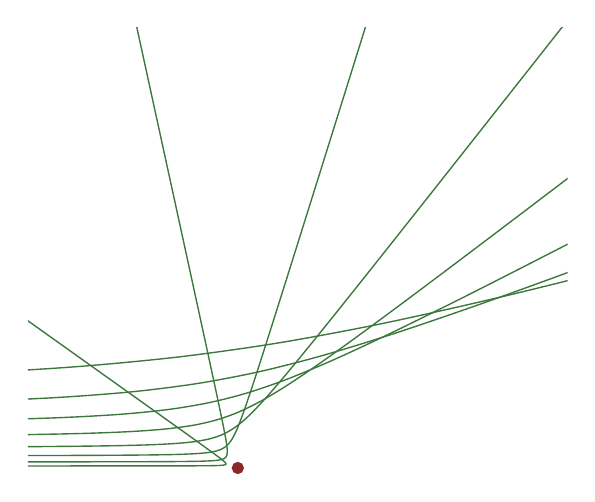
\begin{tikzpicture}[scale=1]
  \message{^^JHyperbolic trajectories}
  
  % limits & parameters
  \def\xa{-35}
  \def\xb{ 55}
  \def\ya{ -1}
  \def\yb{ 55}
  \def\tmax{5}
  \def\N{30} % number of points
  
  \begin{axis}[ xmin=\xa,xmax=\xb,
                ymin=\ya,ymax=\yb,
                hide x axis, hide y axis,
              ]
    \def\a{1}
    \foreach \u in {1,3,6,10,15,21,28,38}{
      \message{^^J  u=\u}
      \def\b{\u*0.25}
      \def\c{sqrt(\a^2+\b^2)}
      \addplot[color=mydarkgreen,line width=0.5,samples=\N,smooth,variable=\t,domain=-\tmax:\tmax]
         ({  \a/\c*(-\a*cosh(\t)-\c) + \b/\c*\b*sinh(\t) },
          { -\b/\c*(-\a*cosh(\t)-\c) + \a/\c*\b*sinh(\t) });
    }
    
    \addplot[mydarkred,mark=*,mark size=2pt,mark options=solid] coordinates {(0,0)};
    
  \end{axis}
  
\end{tikzpicture}


% RUTHERFORD SCATTERING - single vs. compound scattering
% http://www.ffn.ub.es/luisnavarro/nuevo_maletin/Rutherford%20(1911),%20Structure%20atom%20.pdf
% https://tex.stackexchange.com/questions/45151/format-numbers-as-a-fraction-of-pi-with-tikz-pgfmathprintnumber
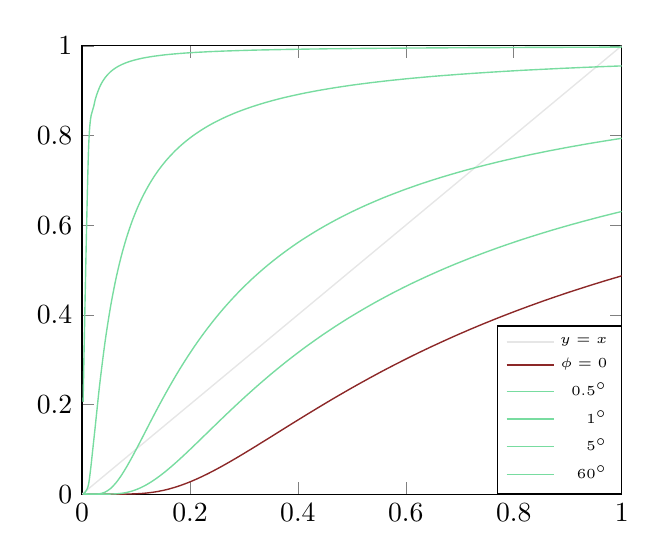
\begin{tikzpicture}[scale=1]
  \message{^^JSingle vs. compound scattering}
  
  % limits & parameters
  \def\xa{0.0}
  \def\xb{1.0}
  \def\ya{0.0}
  \def\yb{1.0}
  \def\A{ 1.0}
  \def\B{ 1.0}
  \def\N{100} % number of points
  
  \begin{axis}[ xmin=\xa,xmax=\xb,
                ymin=\ya,ymax=\yb,
                legend cell align=right,
                legend style={
                  at={(1.0,0.0)},
                  anchor=south east,
                  font=\fontsize{5}{6}\selectfont
                }
              ]
    \addplot[color=mylightgrey,line width=0.5,samples=2,variable=\x,domain=0:1]
      (\x,\x);
    \addlegendentryexpanded{$y=x$}
    
    \addplot[color=mydarkred,line width=0.5,samples=\N,variable=\px,domain=0:1]
      ({ \px },{ \A*exp(-0.72/(\B*\px)) });
    \addlegendentryexpanded{$\phi=0$}
    
    \foreach \ang in {0.5,1,5,60}{
      \message{^^J  ang=\ang}
      \def\myphi{pi*\ang/180}
      \addplot[color=mygreen,line width=0.5,samples=\N,smooth,variable=\px,domain=0.002:1]
        ({ \px },{ \A*exp(-0.181*\myphi^2*cot(\myphi/2 r)^2/(\B*\px)) }); %*cot(\phi/2)^2
      \addlegendentryexpanded{\ang$^\circ$}
      %\addplot[color=mygreen,line width=0.5,samples=\N,smooth,variable=\px,domain=0:1,forget plot]
      %  ({ \px },{ exp(-0.181*\myphi^2*cot(\myphi/2 r)^2/\px) }); %*cot(\phi/2)^2
    }
    
  \end{axis}
  
\end{tikzpicture}


\end{document}
